\documentclass[twoside]{book}

% Packages required by doxygen
\usepackage{fixltx2e}
\usepackage{calc}
\usepackage{doxygen}
\usepackage[export]{adjustbox} % also loads graphicx
\usepackage{graphicx}
\usepackage[utf8]{inputenc}
\usepackage{makeidx}
\usepackage{multicol}
\usepackage{multirow}
\PassOptionsToPackage{warn}{textcomp}
\usepackage{textcomp}
\usepackage[nointegrals]{wasysym}
\usepackage[table]{xcolor}

% Font selection
\usepackage[T1]{fontenc}
\usepackage[scaled=.90]{helvet}
\usepackage{courier}
\usepackage{amssymb}
\usepackage{sectsty}
\renewcommand{\familydefault}{\sfdefault}
\allsectionsfont{%
  \fontseries{bc}\selectfont%
  \color{darkgray}%
}
\renewcommand{\DoxyLabelFont}{%
  \fontseries{bc}\selectfont%
  \color{darkgray}%
}
\newcommand{\+}{\discretionary{\mbox{\scriptsize$\hookleftarrow$}}{}{}}

% Page & text layout
\usepackage{geometry}
\geometry{%
  a4paper,%
  top=2.5cm,%
  bottom=2.5cm,%
  left=2.5cm,%
  right=2.5cm%
}
\tolerance=750
\hfuzz=15pt
\hbadness=750
\setlength{\emergencystretch}{15pt}
\setlength{\parindent}{0cm}
\setlength{\parskip}{3ex plus 2ex minus 2ex}
\makeatletter
\renewcommand{\paragraph}{%
  \@startsection{paragraph}{4}{0ex}{-1.0ex}{1.0ex}{%
    \normalfont\normalsize\bfseries\SS@parafont%
  }%
}
\renewcommand{\subparagraph}{%
  \@startsection{subparagraph}{5}{0ex}{-1.0ex}{1.0ex}{%
    \normalfont\normalsize\bfseries\SS@subparafont%
  }%
}
\makeatother

% Headers & footers
\usepackage{fancyhdr}
\pagestyle{fancyplain}
\fancyhead[LE]{\fancyplain{}{\bfseries\thepage}}
\fancyhead[CE]{\fancyplain{}{}}
\fancyhead[RE]{\fancyplain{}{\bfseries\leftmark}}
\fancyhead[LO]{\fancyplain{}{\bfseries\rightmark}}
\fancyhead[CO]{\fancyplain{}{}}
\fancyhead[RO]{\fancyplain{}{\bfseries\thepage}}
\fancyfoot[LE]{\fancyplain{}{}}
\fancyfoot[CE]{\fancyplain{}{}}
\fancyfoot[RE]{\fancyplain{}{\bfseries\scriptsize Generated by Doxygen }}
\fancyfoot[LO]{\fancyplain{}{\bfseries\scriptsize Generated by Doxygen }}
\fancyfoot[CO]{\fancyplain{}{}}
\fancyfoot[RO]{\fancyplain{}{}}
\renewcommand{\footrulewidth}{0.4pt}
\renewcommand{\chaptermark}[1]{%
  \markboth{#1}{}%
}
\renewcommand{\sectionmark}[1]{%
  \markright{\thesection\ #1}%
}

% Indices & bibliography
\usepackage{natbib}
\usepackage[titles]{tocloft}
\setcounter{tocdepth}{3}
\setcounter{secnumdepth}{5}
\makeindex

% Hyperlinks (required, but should be loaded last)
\usepackage{ifpdf}
\ifpdf
  \usepackage[pdftex,pagebackref=true]{hyperref}
\else
  \usepackage[ps2pdf,pagebackref=true]{hyperref}
\fi
\hypersetup{%
  colorlinks=true,%
  linkcolor=blue,%
  citecolor=blue,%
  unicode%
}

% Custom commands
\newcommand{\clearemptydoublepage}{%
  \newpage{\pagestyle{empty}\cleardoublepage}%
}

\usepackage{caption}
\captionsetup{labelsep=space,justification=centering,font={bf},singlelinecheck=off,skip=4pt,position=top}

%===== C O N T E N T S =====

\begin{document}

% Titlepage & ToC
\hypersetup{pageanchor=false,
             bookmarksnumbered=true,
             pdfencoding=unicode
            }
\pagenumbering{roman}
\begin{titlepage}
\vspace*{7cm}
\begin{center}%
{\Large My Final Assignment \\[1ex]\large 4519089 }\\
\vspace*{1cm}
{\large Generated by Doxygen 1.8.11}\\
\end{center}
\end{titlepage}
\clearemptydoublepage
\tableofcontents
\clearemptydoublepage
\pagenumbering{arabic}
\hypersetup{pageanchor=true}

%--- Begin generated contents ---
\chapter{Namespace Index}
\section{Namespace List}
Here is a list of all namespaces with brief descriptions\+:\begin{DoxyCompactList}
\item\contentsline{section}{\hyperlink{namespaceinterface}{interface} }{\pageref{namespaceinterface}}{}
\end{DoxyCompactList}

\chapter{File Index}
\section{File List}
Here is a list of all files with brief descriptions\+:\begin{DoxyCompactList}
\item\contentsline{section}{scripts/\hyperlink{interface_8py}{interface.\+py} }{\pageref{interface_8py}}{}
\item\contentsline{section}{src/\hyperlink{random__service_8cpp}{random\+\_\+service.\+cpp} }{\pageref{random__service_8cpp}}{}
\end{DoxyCompactList}

\chapter{Namespace Documentation}
\hypertarget{namespaceinterface}{}\section{interface Namespace Reference}
\label{namespaceinterface}\index{interface@{interface}}
\subsection*{Functions}
\begin{DoxyCompactItemize}
\item 
def \hyperlink{namespaceinterface_aca432e6f81aa933df57e2bea65335ee6}{current\+\_\+position} (odom\+\_\+data)
\begin{DoxyCompactList}\small\item\em Read the current position of the robot from odom. \end{DoxyCompactList}\item 
def \hyperlink{namespaceinterface_ac84656acec70183a4ef276f4a3343971}{main} ()
\begin{DoxyCompactList}\small\item\em Takes command from the user and execute the task requested. \end{DoxyCompactList}\item 
def \hyperlink{namespaceinterface_a26cef342aa268117ce542f3465fb6ca0}{move\+\_\+to} (x\+\_\+target, y\+\_\+target)
\begin{DoxyCompactList}\small\item\em Publish the target in order to use move\+\_\+base service to reach it. \end{DoxyCompactList}\item 
def \hyperlink{namespaceinterface_a25416d5ac5c4bc27d42f46875bff174e}{reach\+\_\+target} (x\+\_\+target, y\+\_\+target)
\begin{DoxyCompactList}\small\item\em Keeps the program in sleep until the target isn\textquotesingle{}t reached it also compute and print the distance. \end{DoxyCompactList}\item 
def \hyperlink{namespaceinterface_a0a4ec201152b53b71d452da030b40784}{take\+\_\+position\+\_\+from\+\_\+user} ()
\begin{DoxyCompactList}\small\item\em Takes one of the possible target from the user. \end{DoxyCompactList}\end{DoxyCompactItemize}
\subsection*{Variables}
\begin{DoxyCompactItemize}
\item 
\hyperlink{namespaceinterface_a13ab2be968e67ac3d7d52e5e25c430c3}{current\+\_\+position} = Point()
\begin{DoxyCompactList}\small\item\em It contains the current robot coordinates. \end{DoxyCompactList}\item 
\hyperlink{namespaceinterface_a1de259b3c06e4f436bbade32c75c9318}{pub\+\_\+goal} = None
\begin{DoxyCompactList}\small\item\em To publish new goals. \end{DoxyCompactList}\item 
\hyperlink{namespaceinterface_ac9f12ff0de8248506bf532b6874750e7}{sub\+\_\+odom} = None
\begin{DoxyCompactList}\small\item\em To read the current position. \end{DoxyCompactList}\item 
\hyperlink{namespaceinterface_a4709d1a9f45323d007767a3b7c4725f5}{pub\+\_\+target\+\_\+reached} = None
\begin{DoxyCompactList}\small\item\em To cancel the target. \end{DoxyCompactList}\end{DoxyCompactItemize}


\subsection{Function Documentation}
\index{interface@{interface}!current\+\_\+position@{current\+\_\+position}}
\index{current\+\_\+position@{current\+\_\+position}!interface@{interface}}
\subsubsection[{\texorpdfstring{current\+\_\+position(odom\+\_\+data)}{current_position(odom_data)}}]{\setlength{\rightskip}{0pt plus 5cm}def interface.\+current\+\_\+position (
\begin{DoxyParamCaption}
\item[{}]{odom\+\_\+data}
\end{DoxyParamCaption}
)}\hypertarget{namespaceinterface_aca432e6f81aa933df57e2bea65335ee6}{}\label{namespaceinterface_aca432e6f81aa933df57e2bea65335ee6}


Read the current position of the robot from odom. 

\index{interface@{interface}!main@{main}}
\index{main@{main}!interface@{interface}}
\subsubsection[{\texorpdfstring{main()}{main()}}]{\setlength{\rightskip}{0pt plus 5cm}def interface.\+main (
\begin{DoxyParamCaption}
{}
\end{DoxyParamCaption}
)}\hypertarget{namespaceinterface_ac84656acec70183a4ef276f4a3343971}{}\label{namespaceinterface_ac84656acec70183a4ef276f4a3343971}


Takes command from the user and execute the task requested. 

1) Reach random target

2) Choose target

3) Follow the wall

4) Stop the robot

Possible targets\+:

(-\/4,-\/3);(-\/4,2);(-\/4,7);(5,-\/7);(5,-\/3);(5,1) \index{interface@{interface}!move\+\_\+to@{move\+\_\+to}}
\index{move\+\_\+to@{move\+\_\+to}!interface@{interface}}
\subsubsection[{\texorpdfstring{move\+\_\+to(x\+\_\+target, y\+\_\+target)}{move_to(x_target, y_target)}}]{\setlength{\rightskip}{0pt plus 5cm}def interface.\+move\+\_\+to (
\begin{DoxyParamCaption}
\item[{}]{x\+\_\+target, }
\item[{}]{y\+\_\+target}
\end{DoxyParamCaption}
)}\hypertarget{namespaceinterface_a26cef342aa268117ce542f3465fb6ca0}{}\label{namespaceinterface_a26cef342aa268117ce542f3465fb6ca0}


Publish the target in order to use move\+\_\+base service to reach it. 

\index{interface@{interface}!reach\+\_\+target@{reach\+\_\+target}}
\index{reach\+\_\+target@{reach\+\_\+target}!interface@{interface}}
\subsubsection[{\texorpdfstring{reach\+\_\+target(x\+\_\+target, y\+\_\+target)}{reach_target(x_target, y_target)}}]{\setlength{\rightskip}{0pt plus 5cm}def interface.\+reach\+\_\+target (
\begin{DoxyParamCaption}
\item[{}]{x\+\_\+target, }
\item[{}]{y\+\_\+target}
\end{DoxyParamCaption}
)}\hypertarget{namespaceinterface_a25416d5ac5c4bc27d42f46875bff174e}{}\label{namespaceinterface_a25416d5ac5c4bc27d42f46875bff174e}


Keeps the program in sleep until the target isn\textquotesingle{}t reached it also compute and print the distance. 

\index{interface@{interface}!take\+\_\+position\+\_\+from\+\_\+user@{take\+\_\+position\+\_\+from\+\_\+user}}
\index{take\+\_\+position\+\_\+from\+\_\+user@{take\+\_\+position\+\_\+from\+\_\+user}!interface@{interface}}
\subsubsection[{\texorpdfstring{take\+\_\+position\+\_\+from\+\_\+user()}{take_position_from_user()}}]{\setlength{\rightskip}{0pt plus 5cm}def interface.\+take\+\_\+position\+\_\+from\+\_\+user (
\begin{DoxyParamCaption}
{}
\end{DoxyParamCaption}
)}\hypertarget{namespaceinterface_a0a4ec201152b53b71d452da030b40784}{}\label{namespaceinterface_a0a4ec201152b53b71d452da030b40784}


Takes one of the possible target from the user. 

Possible targets\+:

(-\/4,-\/3);(-\/4,2);(-\/4,7);(5,-\/7);(5,-\/3);(5,1) 

\subsection{Variable Documentation}
\index{interface@{interface}!current\+\_\+position@{current\+\_\+position}}
\index{current\+\_\+position@{current\+\_\+position}!interface@{interface}}
\subsubsection[{\texorpdfstring{current\+\_\+position}{current_position}}]{\setlength{\rightskip}{0pt plus 5cm}interface.\+current\+\_\+position = Point()}\hypertarget{namespaceinterface_a13ab2be968e67ac3d7d52e5e25c430c3}{}\label{namespaceinterface_a13ab2be968e67ac3d7d52e5e25c430c3}


It contains the current robot coordinates. 

\index{interface@{interface}!pub\+\_\+goal@{pub\+\_\+goal}}
\index{pub\+\_\+goal@{pub\+\_\+goal}!interface@{interface}}
\subsubsection[{\texorpdfstring{pub\+\_\+goal}{pub_goal}}]{\setlength{\rightskip}{0pt plus 5cm}interface.\+pub\+\_\+goal = None}\hypertarget{namespaceinterface_a1de259b3c06e4f436bbade32c75c9318}{}\label{namespaceinterface_a1de259b3c06e4f436bbade32c75c9318}


To publish new goals. 

\index{interface@{interface}!pub\+\_\+target\+\_\+reached@{pub\+\_\+target\+\_\+reached}}
\index{pub\+\_\+target\+\_\+reached@{pub\+\_\+target\+\_\+reached}!interface@{interface}}
\subsubsection[{\texorpdfstring{pub\+\_\+target\+\_\+reached}{pub_target_reached}}]{\setlength{\rightskip}{0pt plus 5cm}interface.\+pub\+\_\+target\+\_\+reached = None}\hypertarget{namespaceinterface_a4709d1a9f45323d007767a3b7c4725f5}{}\label{namespaceinterface_a4709d1a9f45323d007767a3b7c4725f5}


To cancel the target. 

\index{interface@{interface}!sub\+\_\+odom@{sub\+\_\+odom}}
\index{sub\+\_\+odom@{sub\+\_\+odom}!interface@{interface}}
\subsubsection[{\texorpdfstring{sub\+\_\+odom}{sub_odom}}]{\setlength{\rightskip}{0pt plus 5cm}interface.\+sub\+\_\+odom = None}\hypertarget{namespaceinterface_ac9f12ff0de8248506bf532b6874750e7}{}\label{namespaceinterface_ac9f12ff0de8248506bf532b6874750e7}


To read the current position. 


\chapter{File Documentation}
\hypertarget{interface_8py}{}\section{scripts/interface.py File Reference}
\label{interface_8py}\index{scripts/interface.\+py@{scripts/interface.\+py}}
\subsection*{Namespaces}
\begin{DoxyCompactItemize}
\item 
 \hyperlink{namespaceinterface}{interface}
\end{DoxyCompactItemize}
\subsection*{Functions}
\begin{DoxyCompactItemize}
\item 
def \hyperlink{namespaceinterface_aca432e6f81aa933df57e2bea65335ee6}{interface.\+current\+\_\+position} (odom\+\_\+data)
\begin{DoxyCompactList}\small\item\em Read the current position of the robot from odom. \end{DoxyCompactList}\item 
def \hyperlink{namespaceinterface_ac84656acec70183a4ef276f4a3343971}{interface.\+main} ()
\begin{DoxyCompactList}\small\item\em Takes command from the user and execute the task requested. \end{DoxyCompactList}\item 
def \hyperlink{namespaceinterface_a26cef342aa268117ce542f3465fb6ca0}{interface.\+move\+\_\+to} (x\+\_\+target, y\+\_\+target)
\begin{DoxyCompactList}\small\item\em Publish the target in order to use move\+\_\+base service to reach it. \end{DoxyCompactList}\item 
def \hyperlink{namespaceinterface_a25416d5ac5c4bc27d42f46875bff174e}{interface.\+reach\+\_\+target} (x\+\_\+target, y\+\_\+target)
\begin{DoxyCompactList}\small\item\em Keeps the program in sleep until the target isn\textquotesingle{}t reached it also compute and print the distance. \end{DoxyCompactList}\item 
def \hyperlink{namespaceinterface_a0a4ec201152b53b71d452da030b40784}{interface.\+take\+\_\+position\+\_\+from\+\_\+user} ()
\begin{DoxyCompactList}\small\item\em Takes one of the possible target from the user. \end{DoxyCompactList}\end{DoxyCompactItemize}
\subsection*{Variables}
\begin{DoxyCompactItemize}
\item 
\hyperlink{namespaceinterface_a13ab2be968e67ac3d7d52e5e25c430c3}{interface.\+current\+\_\+position} = Point()
\begin{DoxyCompactList}\small\item\em It contains the current robot coordinates. \end{DoxyCompactList}\item 
\hyperlink{namespaceinterface_a1de259b3c06e4f436bbade32c75c9318}{interface.\+pub\+\_\+goal} = None
\begin{DoxyCompactList}\small\item\em To publish new goals. \end{DoxyCompactList}\item 
\hyperlink{namespaceinterface_ac9f12ff0de8248506bf532b6874750e7}{interface.\+sub\+\_\+odom} = None
\begin{DoxyCompactList}\small\item\em To read the current position. \end{DoxyCompactList}\item 
\hyperlink{namespaceinterface_a4709d1a9f45323d007767a3b7c4725f5}{interface.\+pub\+\_\+target\+\_\+reached} = None
\begin{DoxyCompactList}\small\item\em To cancel the target. \end{DoxyCompactList}\end{DoxyCompactItemize}

\hypertarget{random__service_8cpp}{}\section{src/random\+\_\+service.cpp File Reference}
\label{random__service_8cpp}\index{src/random\+\_\+service.\+cpp@{src/random\+\_\+service.\+cpp}}
{\ttfamily \#include \char`\"{}ros/ros.\+h\char`\"{}}\\*
{\ttfamily \#include \char`\"{}causa\+\_\+final\+\_\+assignment/\+Random.\+h\char`\"{}}\\*
{\ttfamily \#include $<$math.\+h$>$}\\*
Include dependency graph for random\+\_\+service.\+cpp\+:
\nopagebreak
\begin{figure}[H]
\begin{center}
\leavevmode
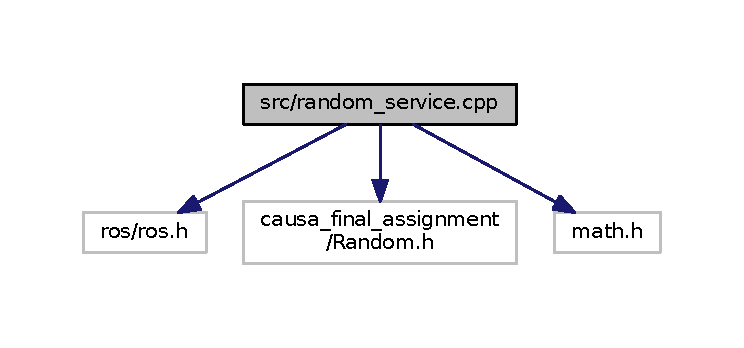
\includegraphics[width=350pt]{random__service_8cpp__incl}
\end{center}
\end{figure}
\subsection*{Functions}
\begin{DoxyCompactItemize}
\item 
bool \hyperlink{random__service_8cpp_ac416fe677dc4867fe3f32f6b47af6f6f}{random\+\_\+pos} (causa\+\_\+final\+\_\+assignment\+::\+Random\+::\+Request \&req, causa\+\_\+final\+\_\+assignment\+::\+Random\+::\+Response \&res)
\begin{DoxyCompactList}\small\item\em Generates random targets among those possible. \end{DoxyCompactList}\item 
int \hyperlink{random__service_8cpp_a3c04138a5bfe5d72780bb7e82a18e627}{main} (int argc, char $\ast$$\ast$argv)
\begin{DoxyCompactList}\small\item\em It defines service /random. \end{DoxyCompactList}\end{DoxyCompactItemize}


\subsection{Function Documentation}
\index{random\+\_\+service.\+cpp@{random\+\_\+service.\+cpp}!main@{main}}
\index{main@{main}!random\+\_\+service.\+cpp@{random\+\_\+service.\+cpp}}
\subsubsection[{\texorpdfstring{main(int argc, char $\ast$$\ast$argv)}{main(int argc, char **argv)}}]{\setlength{\rightskip}{0pt plus 5cm}int main (
\begin{DoxyParamCaption}
\item[{int}]{argc, }
\item[{char $\ast$$\ast$}]{argv}
\end{DoxyParamCaption}
)}\hypertarget{random__service_8cpp_a3c04138a5bfe5d72780bb7e82a18e627}{}\label{random__service_8cpp_a3c04138a5bfe5d72780bb7e82a18e627}


It defines service /random. 

\index{random\+\_\+service.\+cpp@{random\+\_\+service.\+cpp}!random\+\_\+pos@{random\+\_\+pos}}
\index{random\+\_\+pos@{random\+\_\+pos}!random\+\_\+service.\+cpp@{random\+\_\+service.\+cpp}}
\subsubsection[{\texorpdfstring{random\+\_\+pos(causa\+\_\+final\+\_\+assignment\+::\+Random\+::\+Request \&req, causa\+\_\+final\+\_\+assignment\+::\+Random\+::\+Response \&res)}{random_pos(causa_final_assignment::Random::Request &req, causa_final_assignment::Random::Response &res)}}]{\setlength{\rightskip}{0pt plus 5cm}bool random\+\_\+pos (
\begin{DoxyParamCaption}
\item[{causa\+\_\+final\+\_\+assignment\+::\+Random\+::\+Request \&}]{req, }
\item[{causa\+\_\+final\+\_\+assignment\+::\+Random\+::\+Response \&}]{res}
\end{DoxyParamCaption}
)}\hypertarget{random__service_8cpp_ac416fe677dc4867fe3f32f6b47af6f6f}{}\label{random__service_8cpp_ac416fe677dc4867fe3f32f6b47af6f6f}


Generates random targets among those possible. 


%--- End generated contents ---

% Index
\backmatter
\newpage
\phantomsection
\clearemptydoublepage
\addcontentsline{toc}{chapter}{Index}
\printindex

\end{document}
